\chapter{Espacios de Sobolev}

A lo largo de los temas 1 y 2, hemos construido una serie de herramientas básicas en la resolución de ciertos modelos matemáticos. A continuación, vamos a enlazar los conceptos vistos anteriormente y desarrollar los primeros modelos de esta asignatura.

\section{Enlace}

Antes de definir los \textit{espacios de Sobolev}, recordemos algunas propiedades del espacio 
\[L^2(a,b)=\displaystyle\{\funcion{f}{(a,b)}{\R}\;:\; \integral{a}{b}{|f(x)|^2dx<+\infty}\displaystyle\}\]
La norma de este espacio venía dada por $\norm{f}_2=\sqrt{\integral{a}{b}{f(x)^2dx}}$ e inducía el siguiente producto escalar: $<f,g>=\integral{a}{b}{f(x)g(x)dx}$ (nótese que no usamos el conjugado de $g$ ya que estamos trabajando sobre $\R$, no sobre $\C$). Además, $L^2(a,b)\subset L^1(a,b)$ ya que 
\[
\integral{a}{b}{f(x)}=\integral{a}{b}{|f(x)|\cdot 1dx}\leq \left(\integral{a}{b}{f(x)^2dx}\right)^{1/2}\left(b-a\right)^{1/2}
\]
donde hemos usado la desigualdad de Schwartz para el último paso. Con estas propiedades en mente, podemos definir el primer espacio de Sobolev:
\[
\sobolev{1}=\conjunto{f\in\lebesgue{2}: f \text{ tiene derivada débil }f' \text{ y } f'\in\lebesgue{2}}
\]
Este espacio tiene la particularidad de que también cuenta con un producto escalar:
\[
<f,g>=\integral{a}{b}{f(x)g(x)dx}+\integral{a}{b}{f'(x)g'(x)dx}
\]
Por supuesto, $\sobolev{1}$ es un espacio de Hilbert con la norma $\norm{f}=\sqrt{\norm{f}^2_2+\norm{f'}_2^2}$. Es importante recordar que si $f\in\sobolev{1}$, no tiene por qué ser continua (como muestra \textit{The devil staircase}), pero podemos elegir un representante continuo en su clase de equivalencia, es decir, $\sobolev{1}\hookrightarrow C[a,b]$. De hecho:
\begin{prop}\label{inclusion continua}
La aplicación inclusión $\funcion{i}{\sobolev{1}}{C[a,b]}$ es continua.
\end{prop}
\begin{proof}
Pendiente.
\end{proof}
Además, si $f\in C^1[a,b]$, tiene derivada clásica, luego también tiene derivada débil, luego $f\in\sobolev{1}$. Resumiendo, hemos construido la siguiente cadena:
\[
C^1[a,b]\subset\sobolev{^1}\subset C[a,b]\subset \lebesgue{2}
\]
Definimos ahora el siguiente espacio de Sobolev:
\[
\sobolev{2}=\conjunto{f\in\lebesgue{2}: \exists f',f''\in\lebesgue{2}\text{ (débiles)}}
\]
Usando la propiedad \ref{derivadanesima}, tenemos que $\sobolev{2}\subset C^1[a,b]$ y repitiendo el argumento anterior $C^2[a,b]\subset \sobolev{2}$, es decir:
\[
C^2[a,b]\subset \sobolev{2}\subset C^1[a,b]
\]
Repitiendo este proceso iterativamente, podemos definir el $n$-ésimo espacio de Sobolev:
\[
\sobolev{n}=\conjunto{f\in\lebesgue{2}: \exists f',\dots,f^{n)}\in\lebesgue{2} \text{ (débiles)}}
\]
con la propiedad:
\[
C^{n}[a,b]\subset\sobolev{n}\subset C^{n-1}[a,b]\subset\sobolev{n-1}\subset\dots\subset\sobolev{1}\subset\lebesgue{2}
\]

¿Qué tienen de particular estos espacios? Que son de Hilbert, es decir, vamos a poder usar todas las herramientes que tenemos de Análisis Funcional para resolver algunos problemas como veremos en los siguientes apartados.

\begin{definition}
Diremos que $\funcion{F}{[a,b]\times\R^2}{\R}$ es una \textit{función de Carathéodory} si cumple:
\begin{enumerate}[(a)]
\item Para casi todo punto $x\in(a,b)$, $F(x,y,p)$ es continua en $(y,p)$.
\item Para casi todo punto $(y,p)\in\R^2$, la función $x\mapsto F(x,y,p)$ es medible.
\item Dado $K\subset[a,b]\times\R^2$ compacto, existe una función $m_k(x)\in\lebesgue{1}$ tal que $\valorabsoluto{F(x,y,p)}\leq m_k(x)$ $\forall(x,y,p)\in K$.
\end{enumerate}
\end{definition}

Para que la teoría que vamos a desarrollar a continuación tenga sentido, vamos a imponer de ahora en adelante que $F$, $F_y$ y $F_p$ sean de Carathéodory. Haciendo uso de la propiedad (c), podemos definir el funcional $\funcion{L}{\sobolev{1}}{\R}$:
\[
L(y)=\integral{a}{b}{F(x,y(x),y'(x))dx}
\]
que está bien definido ya que que $F$ es medible y está acotada por una función que es integrable. Tomando $\phi\in\soportecompacto$, podemos definir otra función $\funcion{g}{[a,b]}{\R}$ por $g(s)=L(y+s\phi)$, derivarla respecto a $s$ y evaluarla en 0 (a esta expresión la llamamos \textit{derivada de y a lo largo de $\phi$}):
\[
g'(0)=DL_y(\phi)=\integral{a}{b}{F_y(x,y(x),y'(x)dx}+\integral{a}{b}{F_p(x,y(x),y'(x)dx}
\]
\newpage

\section{Modelos de cuerdas}

Procedemos a la introducción del \textit{modelo de cuerdas}. Comenzaremos realizando el planteamiento más simple, densidad constante y extremos fijos. Posteriormente, eliminaremos la primera hipótesis y resolveremos dos casos: en el primero partimos de una función de densidad dada explícitamente. Por el contrario, en el segundo caso, lo resolveremos dada una función de densidad arbitraria. A continuación, supondremos que el puente se haya \textit{sujeto} por varias cuerdas elásticas. Finalmente, supondremos fijos los extremos.

Aunque ya hemos desarrollado una cantidad de resultados considerable, todavía precisamos de ciertos resultados, mayoritariamente del \textit{Análisis Funcional}, que iremos introduciendo al mismo tiempo que el modelo. Como estamos trabajando sobre espacios de Sobolev, que son de Hilbert, podremos usarlos sin mucha complicación.

\subsection{Extremos fijos y densidad constante}

Supongamos tener una \textit{cuerda elástica}, colgada entre dos puntos, 0 y 1, es decir, nuestra cuerda está representada por una función $\funcion{y}{[0,1]}{\R}$ en $\sobolev{1}$ tal que $y(0)=y(1)=1$. El objetivo del modelo será encontrar la \textit{cuerda} de mínima energía. En este caso, vamos a suponer que la \textit{densidad} de la cuerda es una constante $m\in\R^+$. 

Denotamos por $E_p$ a la energía potencial y por $E_e$ a la energía elástica:
\[
E_e=\frac{1}{2}\integral{0}{1}{y'(x)^2dx} \espacio\espacio E_p=\integral{0}{1}{my(x)dx}
\]
Minimizar la energía total de la cuerda, es lo mismo que minimizar el funcional:
\[
L(y)=\frac{1}{2}\integral{0}{1}{y'(x)^2dx}+\integral{0}{1}{my(x)dx}
\]
Usando la notación usual:
\[
L(y)=\integral{0}{1}{F(x,y,p)dx} \; \text{ donde } \;\; F(x,y,p)=\frac{1}{2}p^2+my
\]
Supongamos que $y\in\sobolev{1}$ es un punto crítico del funcional $L:\sobolev{1}\longrightarrow\R$ para poder usar la teoría de la \textit{ecuación de Euler}.
Si calculamos las derivadas parciales de $F(x,y,p)$:
\[
Z(x)=F_p(x,y,p)=p=y'(x) \espacio Z'(x)=F_y(x,y,p)=m
\]
vemos que $Z(x)$ tiene derivada débil ($Z'(x)$), como consecuencia, $y'(x)$ es continua (proposición \ref{representantecontinuo}). Pero además, $Z'(x)=(y'(x))'=y''(x)=m$, continua, por lo tanto $y\in C^2[0,1]$. En resumen, tenemos que resolver la siguiente EDO de segundo orden:
\[
\left\{
\begin{array}{rl}
y''(x) & = m \\
y(0) & = 0 \\
y(1) & = 0
\end{array}
\right.
\]
Si recordamos algo de ecuaciones diferenciales, nos damos cuenta de que las condiciones iniciales están \textit{mal planteadas}. Para poder resolver la ecuación, necesitamos dos conciones sobre el mismo punto: una en $y$ y otra en $y'$. Lo podemos solucionar usando el llamado \textit{método de tiro}, que consiste en darle un valor arbitrario a la condición que nos falta, resolver la ecuación y despejar el valor posteriormente. Asumiendo que $y'(0)=\alpha\in\R$, nos queda:
\[
\left\{
\begin{array}{rl}
y''(x) & = m \\
y'(0) & = \alpha \\
y(0) & = 0
\end{array}
\right.
\]
con solución $y(x)=\integral{0}{x}{\left(\alpha+msds\right)}=m\frac{x^2}{2}+\alpha x$. Usando $y(1)=0$, obtenemos que $\alpha=-\frac{m}{2}$. Por lo que la solución del modelo es:
\[
y(x)=\frac{m}{2}x(x-1) \;\; \forall x \in[0,1]
\] 

\subsection{Extremos fijos y densidad no constante}

El planteamiento es igual al anterior, pero suponemos que la densidad en lugar de ser constante es la función $\funcion{q}{[0,1]}{\R}$ dada por:
\[
q(x)=\left\{\begin{array}{cc}
1 & x \in[0,\frac{1}{2}] \\
\frac{1}{2} & x \in(\frac{1}{2}, 1] 
\end{array}
\right.
\]
Cabe resaltar que $q(x)$ no es continua (presenta un salto en $x=\frac{1}{2}$, pero no importa a la hora de resolverlo. En este caso, el funcional viene dado por:
\[
L(y)=\integral{0}{1}{\frac{1}{2}y'(x)^2+q(x)y(x)dx}
\]
con $F(x,y,p)=\frac{1}{2}p^2+q(x)y$, $F_p(x,y,p)=p$, $F_y(x,y,p)=q(x)$. La ecuación diferencial a resolver es (usando de nuevo el método de tiro):
\[
\left\{
\begin{array}{rl}
y''(x) & = q(x) \\
y(0)  = 0,y'(0) & = \alpha \\
y(1)= 0, y'(1) & = \beta
\end{array}
\right.
\]
Tenemos el problema de que $y\notin C^2[0,1]$. Intentemos arreglarlo:
\begin{itemize}
\item Si $x\in(0,\frac{1}{2}) \Rightarrow y''(x)=1 \Rightarrow y\in C^2(0,\frac{1}{2}) \Rightarrow y'(x)=\integral{0}{x}{1dx}+y'(0)=x+\alpha$\\
 $\Rightarrow y(x)=\integral{0}{x}{x+\alpha dx}=\frac{x^2}{2}+x\alpha$.
\item Si $x\in(\frac{1}{2},1) \Rightarrow y''(x)=1/2 \Rightarrow y\in C^2(\frac{1}{2},1) \Rightarrow y'(x)=y'(1)-\integral{x}{1}{\frac{1}{2}dx}=\beta+\frac{x}{2}-\frac{1}{2}$\\
$\Rightarrow y(1)-y(x)=\integral{x}{1}{\frac{x}{2}-\frac{1}{2}+\beta dx}\Rightarrow y(x)=\frac{x^2}{2}-\frac{x}{2}+\beta(x-1)+\frac{1}{4}$
\end{itemize}
Quedando:
\begin{equation}\label{y}
y(x)=\left\{
\begin{array}{cc}
\frac{x^2}{2}+x\alpha & x\in[0,1/2]) \\
\frac{x^2}{2}-\frac{x}{2}+\beta(x-1)+\frac{1}{4} & x\in(1/2,1]
\end{array}
\right.
\end{equation}

\begin{equation}\label{yprima}
y'(x)=\left\{
\begin{array}{cc}
x+\alpha & x\in[0,1/2]) \\
\frac{x}{2}-\frac{1}{2}+\beta & x\in(1/2,1]
\end{array}
\right.
\end{equation}

Ahora tenemos que resolver el sistema de $\alpha$ y $\beta$. Obtendremos dos ecuaciones de imponer que $y$ e $y'$ sean continuas en $\frac{1}{2}$, es decir, de que las dos partes evaluadas en ese punto coincidan. Por lo que a partir de \eqref{y} y \eqref{yprima} conseguimos,evaluando en $\frac{1}{2}$ e igualando:
\begin{equation}
\left\{
\begin{array}{cc}
\alpha+\beta & =0 \\
\alpha-\beta & =-\frac{3}{4}
\end{array}
\right.
\end{equation}
Resolviendo el sistema, $\alpha=-\frac{3}{8}$, $\beta=\frac{3}{8}$. Quedando finalmente la siguiente solución al modelo: (esta mal)
\begin{equation}\label{y}
y(x)=\left\{
\begin{array}{cc}
\frac{x^2}{2}-\frac{x}{4} & x\in[0,1/2]) \\
\frac{x^2}{2}-\frac{x}{2}+\frac{1}{4} & x\in(1/2,1]
\end{array}
\right.
\end{equation}

\begin{figure}[h]
   \center
  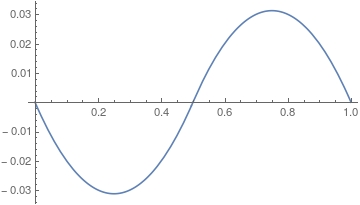
\includegraphics[scale=0.6]{img/puenteflotante.png}
\end{figure}

Que como vemos, floa, asi que algo hay mal :D.

\subsection{Extremos fijos y densidad arbitraria}

El planteamiento es igual al case más simple, pero ahora la función de densidad, $q(x)$, la consideraremos en $C^\infty$. Para evitar tener que explicitar las condiciones de contorno cada vez, es común definir el siguiente subespacio:
\[
\sobolevcero[a,b]{1}=\conjunto{y\in\sobolev{1}: y(a)=y(b)=0}
\]
Recordemos que en este espacio están las funciones de $\lebesgue{2}$, que tienen derivada débil. Por lo tanto, por la proposición \ref{representantecontinuo} podemos elegir una $y$ que sea continua.
\begin{prop}
El espacio vectorial $\sobolevcero{1}$, es cerrado.
\end{prop}   
\begin{proof}
Sea una secuencia de funciones convergentes en $\sobolevcero{1}$, $f_n\longrightarrow f$. Usando la proposición \ref{inclusion continua} y $\sobolevcero{1}\subset\sobolev{1}$, tenemos que $f_n(a)\longrightarrow f(a)$ y $f_n(b)\longrightarrow f(b)$. Luego $f_n(a)=f_n(b)=0 \;\forall n\in\N \Rightarrow f(a)=f(b)=0 \Rightarrow f\in\sobolevcero{1}$.\\
\end{proof}

Una vez definido nuestro nuevo espacio, pasamos a resolver el modelo. Como de costumbre, suponemos que $\in\sobolevcero[0,1]{1}$ es extremal y usamos la teoría de Euler:
\[
L(y)=\frac{1}{2}\integral{0}{1}{y'(x)^2dx}+\integral{0}{1}{q(x)y(x)dx}
\]
Usando la notación usual:
\[
L(y)=\integral{0}{1}{F(x,y,p)dx} \; \text{ donde } \;\; F(x,y,p)=\frac{1}{2}p^2+q(x)y
\]
Calculando sus derivadas parciales
\[
F_p(x,y,p)=p \espacio F_y(x,y,p)=q(x)
\]
podemos calcular $\funcion{DL_y}{\sobolevcero[0,1]{1}}{\R}$ y usar la concidición de extremal de $y$ (teorema \ref{theorem:1.7}):
\[
DL_y(\phi)=\integral{0}{1}{y'(x)\phi'(x)dx}+\integral{0}{1}{q(x)\phi(x)dx}=0 \espacio \forall \phi\in\sobolevcero[0,1]{1}
\]
Si lo miramos como una derivada débil, vemos que si $Z(x)=y'(x) \Rightarrow Z'(x)=q(x) \Rightarrow y''(x)=q(x)$, en sentido débil.
\begin{definition}
$y\in\sobolevcero{1}$ es \textit{solución débil} de $y''(x)=q(x) \; \forall x \in [a,b]$
\end{definition}